\documentclass[11pt]{article}
\pdfminorversion=7
\usepackage[utf8]{inputenc}
\usepackage[T1]{fontenc}
\usepackage[english]{babel}
\usepackage{lmodern,microtype}
\usepackage[a4paper,margin=25mm]{geometry}
\usepackage{amsmath,amssymb,bm,graphicx,booktabs,array,tabularx}
\usepackage[round,authoryear]{natbib}
\usepackage{enumitem,placeins,xcolor}
\usepackage[colorlinks=true,linkcolor=blue!45!black,citecolor=blue!45!black,urlcolor=blue!45!black]{hyperref}
\usepackage{caption,xurl}
\captionsetup{font=small,labelfont=bf}
\setlength{\parskip}{4pt}
\setlength{\parindent}{1em}
\setlength{\emergencystretch}{2em}
\setlength{\textfloatsep}{16pt}
\renewcommand{\topfraction}{0.9}
\renewcommand{\bottomfraction}{0.8}
\renewcommand{\textfraction}{0.08}
\renewcommand{\floatpagefraction}{0.45}
\setcounter{topnumber}{3}
\setcounter{totalnumber}{5}
\raggedbottom
\graphicspath{{figures/}{legacy_figures/}}
\newcommand{\E}{\operatorname{E}}
\newcommand{\Var}{\operatorname{Var}}
\newcommand{\diag}{\operatorname{diag}}

\title{Bayesian spectral selection for road-segment crash counts:\\road attributes and length sensitivity}
\author{Danna L. Cruz-Reyes\thanks{Corresponding author: \href{mailto:dlcruzr@unal.edu.co}{dlcruzr@unal.edu.co}. Departamento de Estad\'istica, Universidad Nacional de Colombia, Bogot\'a, Colombia.}
\and Juan Sosa\thanks{Departamento de Estad\'istica, Universidad Nacional de Colombia, Bogot\'a, Colombia.}
\and Carlos A. Mart\'inez\thanks{Departamento de Producci\'on Animal, Universidad Nacional de Colombia, Bogot\'a, Colombia.}}
\date{}
\begin{document}
\maketitle
\begin{abstract}
Crash counts recorded on road segments require spatial representations that respect network connectivity and distinguish residual patterns from observed road characteristics. We develop a Bayesian negative-binomial model using graph-derived spectral columns on the segment support and an eigenvalue-informed continuous spike-and-slab prior with ordered component scales. Posterior slab-membership probabilities describe component-specific evidence without imposing exact-zero coefficients. Applications to prepared networks in Barcelona and Bogot\'a compare adjustment for road class, lane count and surface tags, followed by sensitivity to the proportionality between counts and segment length. Among 20 candidate modes, expected slab membership decreases from 6.92 to 1.31 in Barcelona and from 4.44 to 2.47 in Bogot\'a after both adjustments. Estimated length elasticities are approximately 0.59 in both networks. No Barcelona mode exceeds a membership probability of 0.5 in the fully adjusted specification; one Bogot\'a mode does, with probability 0.56. Nevertheless, retaining the continuous spectral field improves exploratory pointwise predictive scores over an otherwise matched nonspatial model. These findings distinguish component membership from predictive spatial contribution and show how length assumptions affect spectral interpretation. Remaining data-provenance checks, predictive discrepancies and comparator sampling warnings limit substantive and out-of-region conclusions. The contribution is a segment-supported framework for examining conditional network patterns and their uncertainty within a fixed candidate basis.
\end{abstract}
\noindent\textbf{Keywords:} geographical information science; road networks; spectral spatial modelling; Bayesian shrinkage; crash counts; observational support

\section{Introduction}
Road-crash observations combine an event process with a geographical representation of the infrastructure on which events are recorded. A segment count is indexed by a line feature, while the connectivity that can induce dependence is determined by intersections and shared endpoints. This creates a GIScience question about observational support: how should a spatial representation preserve the topology of the road network while remaining aligned with the units entering the likelihood? A second question concerns interpretation. A broad network pattern may reflect unobserved spatial variation, recorded road characteristics, or an assumption about how counts accumulate with segment length. Distinguishing these possibilities is necessary before interpreting a spectral map as residual spatial information.

Bayesian spatial models have long been used for roadway counts and crash mapping \citep{song2006,aguerovalverde2008}. Intersection-based applications represent corridor dependence or interactions among closely spaced junctions \citep{guo2010,xie2014}. Segment models and joint segment--intersection models recognize that the appropriate support depends on the response being analysed \citep{aguerovalverde2008,zenghuang2014}. When a segment response is explained by a latent intersection field, a projection from nodes to edges is additionally required. Defining the field directly on segments avoids that projection, although it does not by itself establish a new class of spatial dependence.

Graph representations also support a broader programme of geographical information modelling. For example, \citet{maduako2019} represent changing relationships among places and events using a space-time varying graph and demonstrate the representation with traffic accidents. Their contribution concerns dynamic graph representation and querying, whereas the present study concerns statistical regularization and interpretation of aggregate segment counts. The common issue is that topology and observational support are substantive modelling choices rather than merely cartographic details.

Eigenvector spatial filtering and graph signal processing provide established ways to express spatial variation using graph-adapted patterns \citep{griffith2003,griffith2019,shuman2013}. Random-effects spectral formulations accommodate uncertainty in the coefficients \citep{murakami2015}, while Bayesian dimension reduction and shrinkage address regularization and interactions with fixed effects \citep{hughes2013,donegan2020}. Thus, neither spectral spatial modelling nor Bayesian shrinkage of eigenvector coefficients is new. The random edge neighbourhood Gaussian model, RENeGe, supplies an existing segment-neighbourhood construction from which a road-supported operator can be obtained \citep{cruzreyes2023spasta}.

We combine that segment support with an eigenvalue-informed continuous mixture prior and posterior membership summaries. The framework is used to ask which candidate network patterns retain evidence after accounting for road attributes and the assumed relationship between counts and segment length. The candidate set is kept fixed within each city so that changes in posterior evidence cannot be attributed to changes in the graph or basis. We compare the mixture formulation with a nonspatial negative-binomial model, a dense low-rank spectral alternative and a spectral BYM2-type comparator.

The empirical contribution has three parts. First, we maintain a transparent distinction between the original operator eigenvectors, the transformed columns entering the regression, and the signed posterior contributions that can be mapped. Second, we examine component membership before and after adjustment for road class, lane count and surface tags, with a further sensitivity analysis estimating the length coefficient. Third, we separate membership evidence, predictive contribution and distributional adequacy. A continuous spike permits nonzero coefficients, so weak slab membership need not imply that the fitted spatial field has no predictive value. These claims concern a fixed low-rank representation; they do not establish superiority over full-rank graph models or alternative shrinkage priors.

\section{Road networks, counts and recorded attributes}
\subsection{Observational support and analytical samples}
The analyses use two supplied spatial datasets containing road geometry, graph objects, OpenStreetMap-derived attributes and a stored segment response. We reconstructed binary segment adjacency from shared endpoints, retained the connected component containing the greatest number of segments, and preserved the original segment order. Parallel road features were retained; a pair sharing both endpoints received one binary adjacency entry. Independent reconstruction of the adjacency directly from the retained geometries reproduced the matrix used in the models. This checks geographical alignment of geometry and graph support, rather than validation of the original crash records.

The Barcelona source contains 2,714 segments. Its retained component has 2,540 segments and 2,028 intersections. The Bogot\'a source contains 8,169 segments; its retained component has 6,079 segments and 5,107 intersections. Component restriction excludes 174 and 2,090 segments, respectively. The resulting inference is conditional on the retained networks. Characteristics of excluded components and sensitivity to the study boundary have not been evaluated. Table~\ref{tab:data} describes only the retained analytical support.

\begin{table}[tb]
\centering\small
\caption{Retained analytical samples. Totals are recovered from the stored segment response; they have not been reconciled with event-level source records.}
\label{tab:data}
\begin{tabular}{lrr}\toprule
Characteristic & Barcelona & Bogot\'a\\\midrule
Retained segments & 2,540 & 6,079 \\
Retained intersections & 2,028 & 5,107 \\
Recovered total count &  3,735 & 85,068 \\
Represented length (km) & 224.9 & 779.0 \\
Zero-count segments (\%) & 54.0 & 28.3 \\
\bottomrule
\end{tabular}
\end{table}

\subsection{Response recovery and provenance}
For each retained segment, the stored response is numerically compatible with $\log(1+Y_e)$ for a nonnegative integer $Y_e$. We inverted this transformation and checked the integer correspondence. Recovered totals are 3,735 for Barcelona and 85,068 for Bogot\'a. This verifies a numerical transformation; it does not verify event deduplication, inclusion criteria or assignment of crashes to segments. In the Bogot\'a source, a separate object named \texttt{Y\_edges} has 54,497 entries and is incompatible with the 8,169 source road features. That object was excluded. The response used here is the geometry-aligned segment column.

The preceding manuscript attributes the Barcelona observations to Open Data BCN over 2010--2015 and the Bogot\'a observations to the municipal crash-data portal. The exact records and observation period represented by the prepared Bogot\'a response remain to be reconciled. These applications are therefore conditional analyses of the supplied prepared counts, not verified estimates of city-wide incidence. The revised Bogot\'a support also differs from the 6,076-segment support reported previously. All numerical results in the main text refer to the present 6,079-segment reconstruction; earlier application estimates are not pooled with them.

Segment lengths were recomputed from the projected geometries: ETRS89/UTM zone 31N for Barcelona and EPSG:3116 for Bogot\'a. Length measures the amount of represented roadway, not vehicle flow. No traffic-volume-adjusted risk is estimated, and different observation periods prevent substantive cross-city comparisons of count levels.

\subsection{Covariate construction}
The common road attributes are road class, lane-count category and surface tag. Road class is recorded for all retained features and has four categories: residential, tertiary, secondary and primary. Residential roads form the reference group. Lane counts are grouped as one, two, three or more, and unknown, with two lanes as reference. A recorded value of 22 in Bogot\'a was flagged as implausible for this analysis and assigned to the unknown category. Unknown lane counts occur on 430 Barcelona segments (16.9\%) and 498 Bogot\'a segments (8.2\%).

Surface tags are grouped as \texttt{asphalt}, another recorded tag, and unknown. Another tag includes generic \texttt{paved} as well as more specific materials; it cannot be interpreted uniformly as absence of asphalt. Only 22 Barcelona segments have another recorded surface tag, compared with 583 in Bogot\'a. Surface is unknown on 138 and 160 segments. Unknown categories are nuisance controls for recording patterns, not observations that the corresponding infrastructure is absent. Complete category counts and coefficient summaries are supplied in the supplementary material.

The attributes have not been harmonized historically with the crash observation periods. Their coefficients are conditional associations within these prepared datasets, not historical causal effects. We avoid selecting additional covariates from incomplete speed or width fields at this stage. Road attributes are introduced as a fixed, interpretable set; they are not selected by the spectral mixture.

\section{A segment-supported spectral representation}
\subsection{From road topology to candidate patterns}
Let $G=(V,E)$ be an undirected road graph and let $n=|E|$ denote the number of retained segments. Define the $n\times n$ binary matrix $A$ by $A_{er}=1$ when distinct segments $e$ and $r$ share an endpoint. Its diagonal is zero. This is a simple edge-neighbourhood, or line-graph, representation of the road network. With $D=\diag(A\bm 1)$, define the symmetric normalized adjacency
\begin{equation}
 S=D^{-1/2}AD^{-1/2}=U\Delta U^{\mathsf T},
 \qquad \Delta=\diag(\delta_1,\ldots,\delta_n).
 \label{eq:operator}
\end{equation}
Eigenvalues lie in $[-1,1]$ and are ordered decreasingly. For a connected retained component, $\delta_1=1$ and the Perron eigenvector is proportional to $D^{1/2}\bm 1$. It is generally not constant. The normalized Laplacian $I-S$ has eigenvalues $1-\delta_j$, so leading adjacency eigenvectors encode low graph-frequency patterns in this normalized representation. The ordering concerns the source eigenvectors and does not assign a physical distance scale to each mode.

We computed the leading 61 eigenpairs for descriptive examination. The largest eigen-equation residual norm was below $6\times10^{-11}$ in both networks. For model fitting, the candidate set is $u_2,\ldots,u_{21}$, with $M=20$ and $\lambda_j=\delta_{j+1}$. All reported candidate indices start at one after omission of Perron. Figure~\ref{fig:spectrum} shows the upper end of the spectrum; Figure~\ref{fig:raw} maps the first three candidate eigenvectors. Only the upper spectrum was computed, so these figures do not describe the full range of network frequencies or justify a global variance-explained claim.

\begin{figure}[tb]\centering
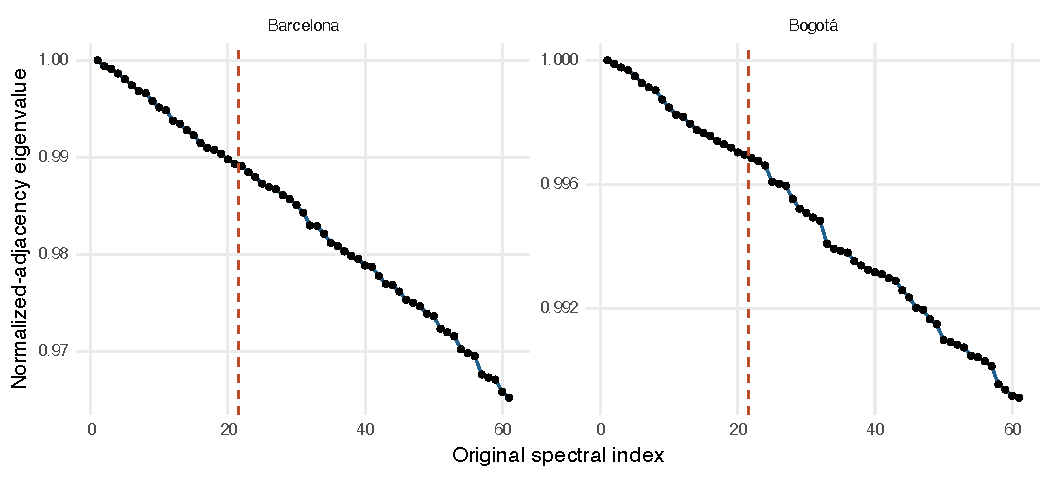
\includegraphics[width=\textwidth]{spectrum.pdf}
\caption{Leading normalized-adjacency eigenvalues. Original index 1 is Perron; indices 2--21 enter the candidate set. The dashed boundary separates fitted candidates from additional eigenpairs computed for description. Vertical scales differ between cities.}
\label{fig:spectrum}\end{figure}
\begin{figure}[p]\centering
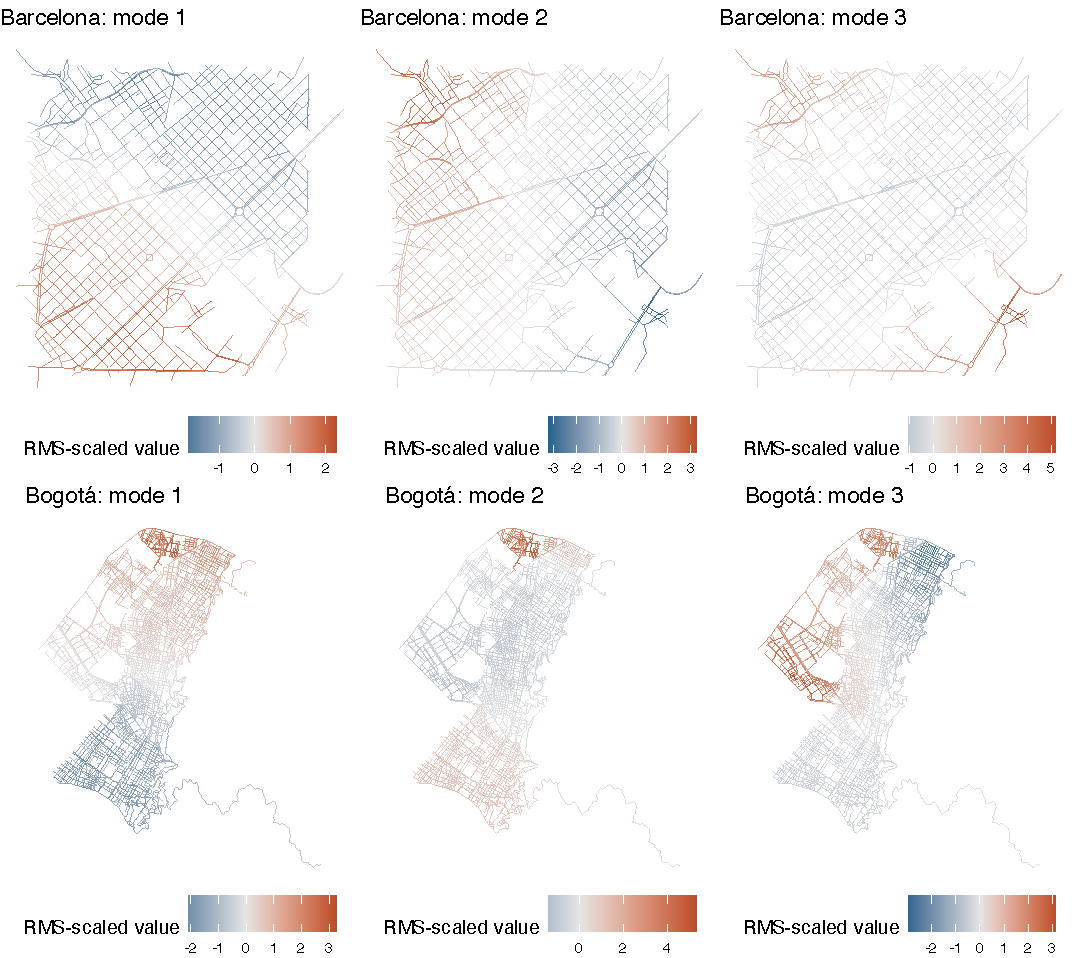
\includegraphics[width=\textwidth]{raw_network_modes.pdf}
\caption{First three candidate eigenvectors in each retained network, scaled to unit root-mean-square without centering. Scalar rescaling preserves their eigenvector property. Signs are arbitrary, and colours represent graph contrasts rather than estimated crash effects. Each panel has its own legend.}
\label{fig:raw}\end{figure}

\subsection{Regression columns and the RENeGe connection}
For $v_j=u_{j+1}$, the fitted column is
\begin{equation}
 B_{ej}=\frac{v_{ej}-\bar v_j}{\{n^{-1}\sum_{r=1}^n(v_{rj}-\bar v_j)^2\}^{1/2}},
 \qquad \bar v_j=n^{-1}\sum_{e=1}^n v_{ej}.
 \label{eq:basis}
\end{equation}
Centering removes the intercept direction and RMS scaling puts coefficient scales on a comparable footing. These operations do not generally preserve mutual orthogonality or the eigenvector property. The fitted field $s=Bb$ is therefore expressed in graph-derived columns whose source ordering is spectral, rather than in an unchanged orthonormal eigenbasis.

The eigenvalue weighting is motivated by the proper edge-neighbourhood precision $Q(\gamma)=\kappa(D-\gamma A)$ \citep{cruzreyes2023spasta}. Its exact covariance is
\begin{equation}
 Q(\gamma)^{-1}=\kappa^{-1}D^{-1/2}U
 \diag\{(1-\gamma\delta_j)^{-1}\}U^{\mathsf T}D^{-1/2}.
\end{equation}
Our regression uses the transformed $B$ and omits the external degree factors. It is an operator-inspired low-rank construction, not an exact reparameterization of this full Gaussian field. Omitting Perron is likewise a modelling restriction: since Perron is degree-related before transformation, omission can remove more than an intercept. These distinctions are important for interpreting what the candidate set can represent.

Eigenvector signs are arbitrary. Consequently, interpretation uses a signed posterior contribution $a_j=B_j\E(b_j\mid Y)$, which is invariant to simultaneously reversing a column and its coefficient. We report its RMS magnitude to rank contributions and map the contributions themselves. This differs from interpreting an unweighted eigenvector as an estimated crash pattern.

\FloatBarrier
\section{Bayesian count model and comparison design}
\subsection{Road attributes and the length assumption}
For segment $e$, let $L_e$ be length in kilometres and $x_e$ the eight indicator variables formed from the recorded road attributes. We use the negative-binomial parameterization
\begin{align}
 Y_e\mid\mu_e,\phi&\sim\operatorname{NegBinomial}_2(\mu_e,\phi),\\
 \log\mu_e&=\log L_e+\alpha+x_e^{\mathsf T}\beta
      +d\{\log L_e-\overline{\log L}\}+s_e,
 \label{eq:count}
\end{align}
where $\Var(Y_e\mid\mu_e,\phi)=\mu_e+\mu_e^2/\phi$. The primary comparison sets $d=0$, imposing proportional accumulation of expected counts with length. The sensitivity analysis estimates $d$, giving the total length elasticity $\ell=1+d$. Centering changes the intercept interpretation, not the elasticity. When $\ell$ is estimated, the target is an expected count conditional on length and recorded attributes; it should not be described as a constant frequency per kilometre.

We assign $\alpha\sim N(0,5^2)$, each recorded-attribute coefficient $\beta_k\sim N(0,0.7^2)$ and $\phi\sim\operatorname{Exponential}(0.5)$, with the exponential expressed by its rate. In the estimated-length analysis $d\sim N(0,0.7^2)$, so $\ell\sim N(1,0.7^2)$. These priors are independent of the full-data empirical mean. Unknown-category coefficients receive the same regularization as other indicators but are not given physical interpretations.

\subsection{Ordered continuous spike-and-slab regularization}
The spatial field in the mixture spectral model is $s=Bb$. For $j=1,\ldots,M$, define latent membership $z_j$ and
\begin{align}
 z_j\mid\pi&\sim\operatorname{Bernoulli}(\pi), & \pi&\sim\operatorname{Beta}(1,4),\\
 b_j\mid z_j=0&\sim N(0,\sigma_0^2), & \sigma_0&=0.05,\\
 b_j\mid z_j=1,\tau&\sim N(0,\sigma_{1j}^2), &
 \sigma_{1j}^2&=\sigma_0^2+\frac{\tau^2}{1-\gamma\lambda_j},\\
 \tau&\sim N^+(0,0.5^2), & \gamma&=0.9.
 \label{eq:mixture}
\end{align}
The additive spike variance ensures an ordered wider component for $\tau>0$. Larger source eigenvalues permit greater slab variance. The resulting prior shrinks coefficients continuously; it does not set them exactly to zero. Membership probabilities
\begin{equation}
 p_j=\Pr(z_j=1\mid Y)
 =\E\left[\frac{\pi f_N(b_j;0,\sigma_{1j}^2)}
 {\pi f_N(b_j;0,\sigma_{1j}^2)+(1-\pi)f_N(b_j;0,\sigma_0^2)}\;\middle|\;Y\right]
\end{equation}
are recovered after integrating the binary indicators out of the sampling target. They measure posterior allocation to the slab, not the probability that a coefficient is nonzero. When the component scales are close, membership is intrinsically less differentiated.

For $K=\sum_jz_j$, $\E(K\mid Y)=\sum_jp_j$. We also compute its posterior distribution by averaging conditional Poisson-binomial distributions across draws. Quantiles of $K$ are therefore distinct from quantiles of the draw-wise sum of conditional membership probabilities. A threshold of 0.5 is used only to summarize membership descriptively. All coefficient draws contribute to posterior fields and predictions, including coefficients allocated predominantly to the continuous spike. Neither $\E(K\mid Y)$ nor the number above 0.5 is a literal rank of the fitted field.

\subsection{Nonspatial, dense spectral and BYM2-type comparisons}
The nonspatial model sets $s=0$. The dense spectral comparator has $b_j=\tau w_j\xi_j$, where $w_j=(1-\gamma\lambda_j)^{-1/2}$, $\xi_j\sim N(0,1)$ and $\tau\sim N^+(0,0.5^2)$. It retains the complete candidate set without mixture membership. Its label denotes the common low-rank operator-derived representation, not a fitted full-rank CAR model.

The BYM2-type comparator combines a scaled structured field and independent segment effects, following the scaling rationale of \citet{riebler2016}. Let $R=B\diag(w_j)$ and
\begin{equation}
 c^2=\exp\left\{\frac{1}{n}\sum_e\log[(RR^{\mathsf T})_{ee}]\right\}.
\end{equation}
With independent standard normal vectors $\xi$ and $v$, its field is
\begin{equation}
 s=\sigma\{\sqrt{\rho}\,R\xi/c+\sqrt{1-\rho}\,v\},\qquad
 \sigma\sim N^+(0,0.5^2),\quad\rho\sim\operatorname{Beta}(0.5,0.5).
\end{equation}
The structured component has unit geometric-mean marginal variance before multiplication by its scale. This is a spectral BYM2-type comparator on the retained basis, not a full-rank BYM2 analysis.

The primary experiment contains four model families, two cities and two attribute specifications: unadjusted (U) and road-attribute adjusted (C), both imposing $\ell=1$. Four additional fits estimate length (L): nonspatial and mixture spectral models in both cities, with the same recorded attributes. This gives 20 fitted specifications. Dense spectral and BYM2-type models with estimated length were not fitted, so the additional L comparison is matched only between nonspatial and mixture spectral models.

\subsection{Computation, prediction and adequacy}
All models were sampled in CmdStan 2.36.0 using four chains. Initial runs used 1,000 warm-up and 1,000 retained iterations per chain, target acceptance 0.99 and maximum tree depth 13. A diagnostic-triggered rerun used 2,000 warm-up and 2,000 retained iterations, target acceptance 0.995 and depth 14. The operational pass criterion required no divergences or depth saturation, maximum rank-normalized $\widehat R\leq1.01$, minimum bulk effective sample size of 400 and minimum chain E-BFMI of 0.3. We monitored mixture probabilities as well as core parameters; BYM2-type fits also included checks of independent effects. Rank and effective-size diagnostics follow the principles described by \citet{vehtari2021}.

Pointwise Pareto-smoothed importance-sampling leave-one-out evaluation uses up to 2,000 evenly spaced posterior draws and relative-efficiency adjustment \citep{vehtari2017}. For BYM2-type prediction, the held-out independent segment effect is integrated against its normal prior, rather than evaluated using that segment's fitted effect. Normal quadrature starts with 30 nodes and is checked against 60 on high-count and control segments; all segment likelihoods are recomputed with 60 nodes if the maximum checked log-density discrepancy exceeds 0.001. The paired standard error of an ELPD difference is computed from its segment-wise differences.

This procedure leaves neighbouring observations available to the shared spatial field. It evaluates interpolation-like prediction on the retained network, not transfer to unseen districts. Segment-wise standard errors do not replace a spatially blocked experiment. Pareto diagnostics are reported alongside scores, and influential observations require exact refits or an alternative validation design before a definitive ranking.

Posterior predictive checks use 400 replicated datasets to examine the mean, variance, zero fraction, maximum and 99th percentile. A further check compares Moran's $I$ for centred Pearson residuals on the segment graph using 100 posterior draws. These are conditional adequacy checks; they address different questions from sampling convergence or out-of-sample scoring. Field maps use posterior means and marginal 90\% intervals, without simultaneous multiplicity adjustment.

\section{Results}
\subsection{Adjustment changes component membership}
Figure~\ref{fig:membership} shows how posterior membership changes while the graph and candidate set remain fixed. In Barcelona, expected slab membership falls from 6.92 under U to 2.27 under C and 1.31 under L. Modes 1, 2, 8 and 15 exceed 0.5 under U; none does after attribute adjustment. Under L, the largest membership probability is only 0.16. This indicates weak allocation to the wider mixture component, not that every spatial coefficient is zero.

In Bogot\'a, expected membership falls from 4.44 to 2.89 and then 2.47. Modes 1, 6 and 14 exceed 0.5 under U. After attribute adjustment, modes 1 and 6 remain above that descriptive threshold, at approximately 0.67 and 0.61. Under L, mode 1 has probability 0.56 and mode 6 decreases to 0.39. The surviving allocation is moderate rather than decisive. The posterior distributions of $K$ are broad (Table~\ref{tab:membership}); point estimates alone would overstate certainty about a compact set.

\begin{figure}[p]\centering
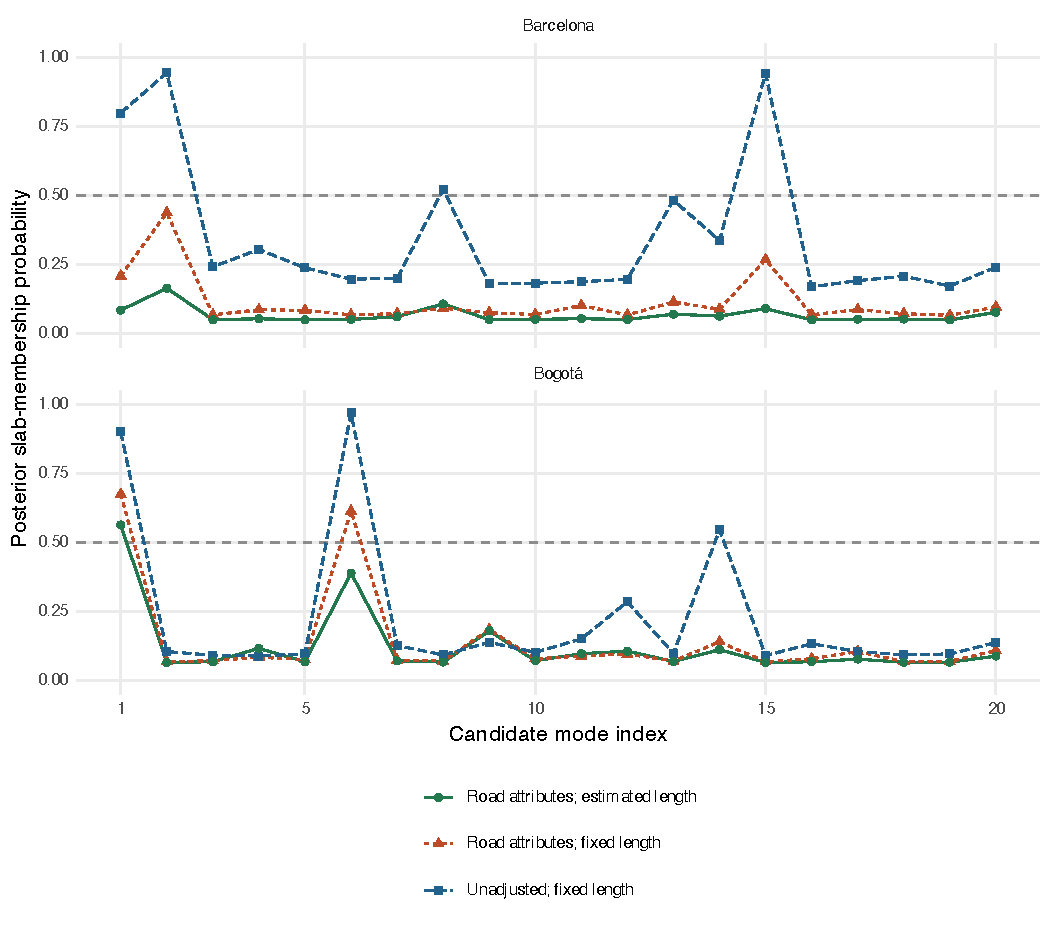
\includegraphics[width=\textwidth]{mode_membership.pdf}
\caption{Posterior slab-membership probabilities for the same 20 candidate columns within each city. U: unadjusted, fixed unit length coefficient; C: recorded road attributes, fixed length coefficient; L: recorded attributes and estimated length coefficient. The dashed 0.5 line is descriptive and is not used to truncate predictions.}
\label{fig:membership}\end{figure}
\begin{table}[tb]\centering\small
\caption{Posterior mixture membership. Intervals refer to the latent membership count $K$, not to an exact number of nonzero regression coefficients. U, C and L are defined in Figure~\ref{fig:membership}.}
\label{tab:membership}
\begin{tabular}{llrcl}\toprule
Network & Specification & $\E(K\mid Y)$ & 90\% interval for $K$ & Modes with $p_j>0.5$\\\midrule
Barcelona & U & 6.92 & [2, 13] & 1, 2, 8, 15 \\
Barcelona & C & 2.27 & [0, 8] & None \\
Barcelona & L & 1.31 & [0, 7] & None \\
Bogotá & U & 4.44 & [1, 9] & 1, 6, 14 \\
Bogotá & C & 2.89 & [0, 8] & 1, 6 \\
Bogotá & L & 2.47 & [0, 8] & 1 \\
\bottomrule
\end{tabular}\end{table}

\FloatBarrier
\subsection{Length sensitivity and recorded road attributes}
In the mixture spectral L model, length elasticities are 0.585 (90\% interval 0.533--0.638) in Barcelona and 0.590 (0.561--0.617) in Bogot\'a. Matched nonspatial estimates are 0.584 (0.531--0.638) and 0.596 (0.567--0.624). Within these specifications, the posterior intervals are well below the imposed unit coefficient. This is evidence against that proportionality assumption in the prepared data, not an estimate of the causal effect of extending a road.

Allowing length to be estimated improves the mixture model's ELPD by 76.3 (paired SE 17.1) in Barcelona and 265.3 (30.3) in Bogot\'a relative to C. The corresponding nonspatial gains are 76.8 (18.5) and 252.3 (29.4). The agreement across spatial and nonspatial fits indicates that the sensitivity is not confined to a particular spatial prior. Differences in traffic volume, segmentation and road function may all contribute to the subproportional association; the available variables cannot separate them.

Table~\ref{tab:effects} reports conditional count ratios from the mixture L models. Comparisons hold recorded attributes and length fixed. They describe associations with the recorded categories; surface-tag comparisons in Barcelona are particularly limited by the small number of alternative recorded tags. Coefficients for unknown categories are retained in estimation and supplied separately, rather than interpreted as infrastructure effects.

\begin{table}[tb]\centering\small
\caption{Conditional count ratios from the mixture spectral model with recorded attributes and estimated length. Values are posterior medians with marginal 90\% intervals. The table excludes nuisance coefficients for unknown categories.}
\label{tab:effects}
\begin{tabular}{p{.42\textwidth}rr}\toprule
Recorded category comparison & Barcelona & Bogot\'a\\\midrule
Tertiary vs residential road & 1.14 [0.95, 1.35] & 1.95 [1.78, 2.13] \\
Secondary vs residential road & 0.97 [0.80, 1.18] & 2.59 [2.36, 2.84] \\
Primary vs residential road & 1.29 [1.04, 1.60] & 3.73 [3.35, 4.17] \\
One vs two lanes & 0.84 [0.69, 1.03] & 1.07 [0.95, 1.20] \\
Three or more vs two lanes & 1.49 [1.27, 1.74] & 1.29 [1.17, 1.43] \\
Other surface tag vs asphalt & 0.86 [0.52, 1.48] & 0.82 [0.73, 0.92] \\
\bottomrule
\end{tabular}\end{table}

\subsection{Signed spatial contributions and uncertainty}
Figure~\ref{fig:contributions} displays the three largest posterior mean contributions by RMS in each L fit. Their ranking differs from ranking membership probabilities: a column can contribute to the field even when its coefficient is predominantly allocated to the continuous spike. The maps display signed combinations of column and coefficient, so their interpretation is unaffected by an arbitrary eigenvector sign reversal. These contributions are conditional log-count contrasts, not traffic-adjusted risk surfaces.

The complete posterior mean fields (Figure~\ref{fig:field}) combine all 20 coefficients. They should not be reconstructed by retaining only the modes above 0.5. Marginal interval maps in the supplementary material identify segments whose field intervals contain zero and distinguish that uncertainty from mixture membership. Such segment-wise intervals do not establish jointly significant hotspot regions. Neither road class nor length adjustment yields a causal decomposition between infrastructure and spatial effects, and collinearity between attributes and graph-derived columns remains possible.

\begin{figure}[p]\centering
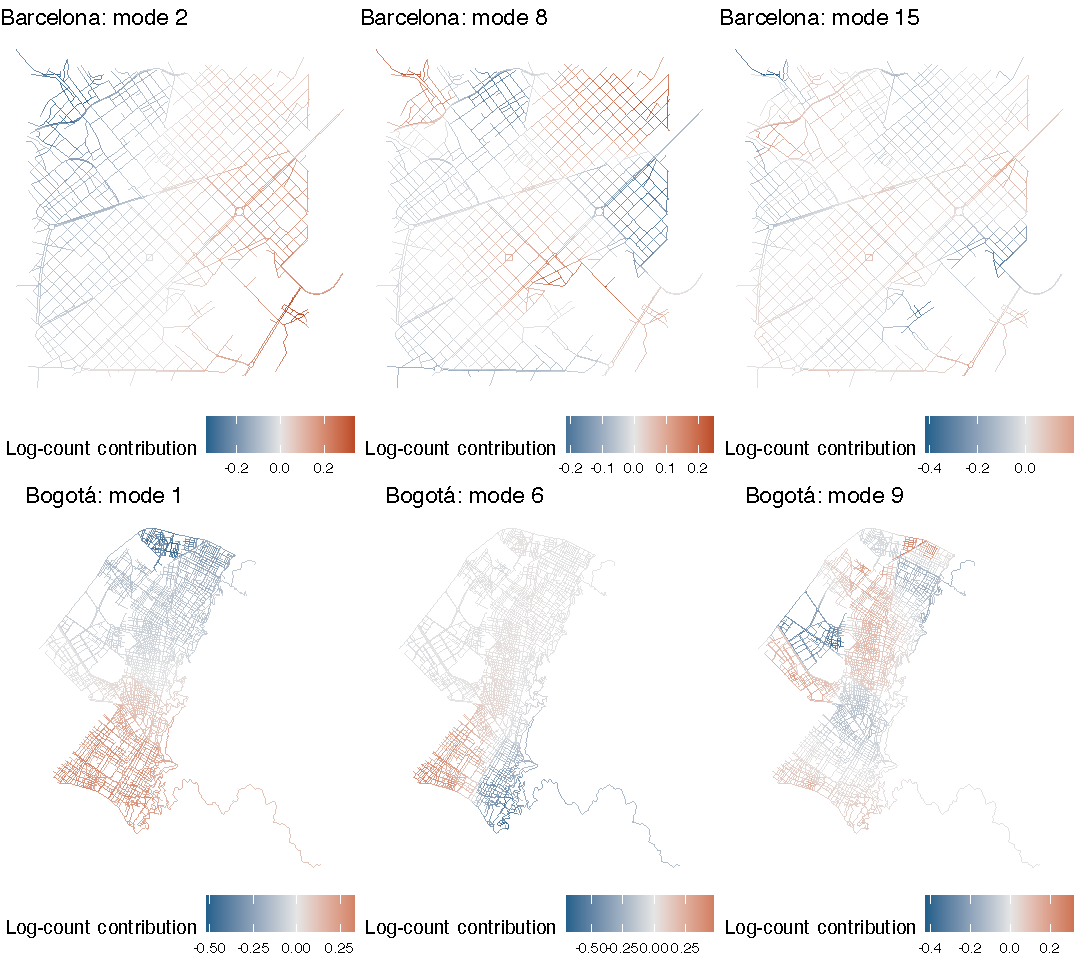
\includegraphics[width=\textwidth]{adjusted_contributions.pdf}
\caption{Three largest RMS posterior mean spectral contributions in each L fit, mapped as $B_j\E(b_j\mid Y)$. Panels have separate colour scales. A displayed contribution does not imply slab membership above 0.5.}
\label{fig:contributions}\end{figure}
\begin{figure}[tb]\centering
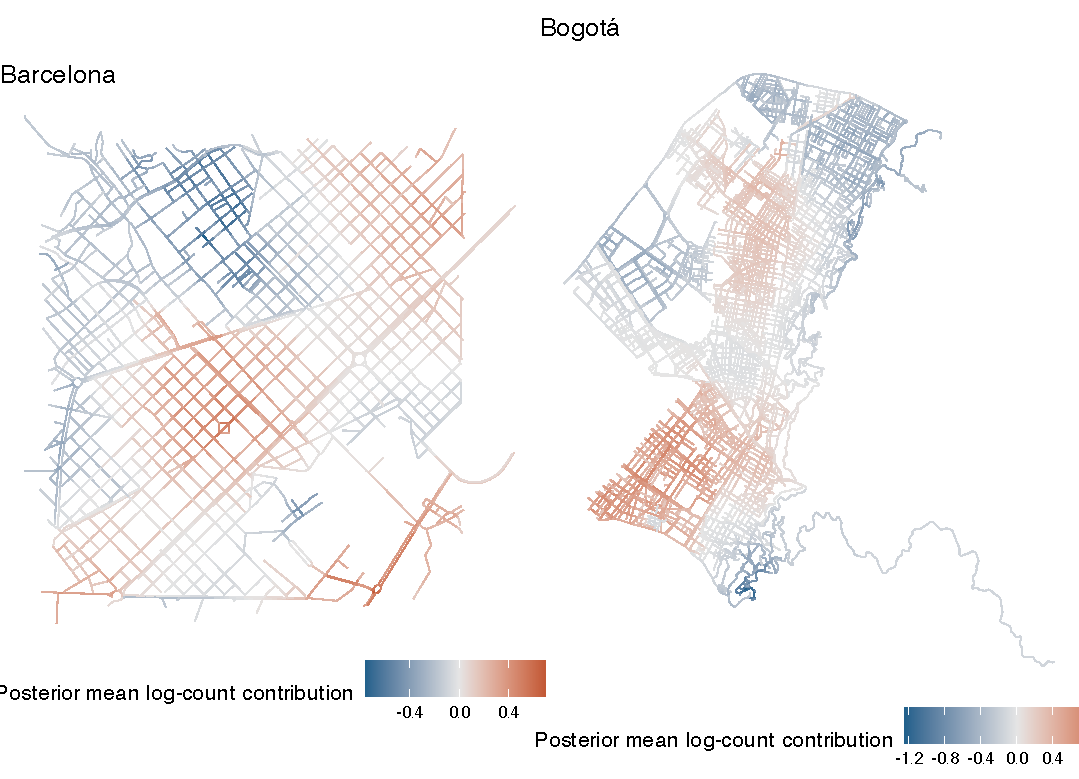
\includegraphics[width=\textwidth]{adjusted_field.pdf}
\caption{Posterior mean structured fields under recorded road attributes and estimated length. Each field combines all candidate coefficients. Colour scales are panel-specific; the maps support within-network conditional interpretation, not comparison of city-level risk.}
\label{fig:field}\end{figure}

\FloatBarrier
\subsection{Predictive contribution and comparator limitations}
The mixture and dense spectral models have almost identical pointwise scores in the matched U and C experiments (Table~\ref{tab:prediction}). Thus, allocation to spike and slab changes the description of component evidence without producing a large advantage over dense regularization on this candidate set. Introducing recorded attributes improves mixture-model ELPD by 36.6 (SE 14.2) in Barcelona and 404.7 (33.8) in Bogot\'a. The direction is consistent across all four model families, although BYM2-type estimates carry sampling warnings.

In the matched L comparison, the mixture spectral model improves on the nonspatial model by 18.1 (SE 7.2) in Barcelona and 95.4 (15.1) in Bogot\'a. This remains compatible with weak slab allocation: the spike is continuous, and the whole posterior field enters prediction. Absence of a membership probability above 0.5 is therefore not a test that all residual spatial information is absent. The Bogot\'a L mixture fit has one influential PSIS observation, with maximum Pareto $k=0.743$, so its predictive gain remains exploratory.

BYM2-type models attain the highest reported scores among the fixed-length specifications. However, all four fail the operational joint sampling criterion after their longer reruns because minimum chain E-BFMI lies between 0.191 and 0.277. Barcelona U also has maximum $\widehat R=1.012$ and minimum bulk ESS 386; Bogot\'a C has minimum bulk ESS 376. There are no divergent transitions or tree-depth saturations in the retained empirical fits. These facts do not eliminate the energy-exploration warnings, and BYM2-type numerical rankings are not treated as definitive evidence of superiority. Their estimated-length versions were not run.

\begin{table}[p]\centering\small
\caption{Exploratory pointwise PSIS-LOO results for all 20 fitted specifications. Higher ELPD is better within the same city. $n_k$ counts segments exceeding the draw-dependent Pareto threshold (approximately 0.697). ``Pass'' refers to the joint sampler criterion, not distributional adequacy. All BYM2-type results are flagged. U and C impose a unit length coefficient; L estimates it.}
\label{tab:prediction}
\begin{tabular}{llrrrl}\toprule
Model & Specification & ELPD & SE & $n_k$ & Sampler\\\midrule
\textit{Barcelona} & & & & &\\
NB & U & -3998.2 & 79.8 & 0 & Pass \\
NB & C & -3931.1 & 81.2 & 0 & Pass \\
NB & L & -3854.3 & 70.7 & 0 & Pass \\
Dense spectral & U & -3949.2 & 78.8 & 0 & Pass \\
Dense spectral & C & -3912.5 & 79.4 & 1 & Pass \\
Mixture spectral & U & -3948.9 & 78.7 & 0 & Pass \\
Mixture spectral & C & -3912.4 & 79.6 & 1 & Pass \\
Mixture spectral & L & -3836.1 & 70.0 & 0 & Pass \\
Spectral BYM2 & U & -3836.7 & 72.5 & 0 & Flagged \\
Spectral BYM2 & C & -3797.1 & 72.3 & 0 & Flagged \\
\addlinespace
\textit{Bogotá} & & & & &\\
NB & U & -20271.9 & 154.8 & 0 & Pass \\
NB & C & -19831.6 & 152.5 & 0 & Pass \\
NB & L & -19579.3 & 141.0 & 0 & Pass \\
Dense spectral & U & -20155.6 & 153.8 & 1 & Pass \\
Dense spectral & C & -19750.0 & 153.1 & 1 & Pass \\
Mixture spectral & U & -20153.9 & 153.7 & 1 & Pass \\
Mixture spectral & C & -19749.2 & 153.0 & 2 & Pass \\
Mixture spectral & L & -19483.9 & 141.3 & 1 & Pass \\
Spectral BYM2 & U & -19848.7 & 141.9 & 0 & Flagged \\
Spectral BYM2 & C & -19421.7 & 141.0 & 0 & Flagged \\
\addlinespace
\bottomrule
\end{tabular}\end{table}

\FloatBarrier
\subsection{Predictive adequacy beyond a score}
Estimating length materially improves calibration of replicated summaries. For Barcelona's mixture L model, the observed mean is 1.470 and the median replicated mean is 1.443, with a 90\% reference interval 1.324--1.567. Observed variance 7.58 is compared with a median replicated variance of 7.89 (6.30--10.68). The observed zero fraction, 0.540, lies within the replicated interval 0.513--0.558. The observed maximum of 26 is at the lower boundary of its replicated interval, indicating remaining upper-tail sensitivity.

In Bogot\'a, the mixture L model reproduces the mean and upper-count summaries more closely than the fixed-length specification. Observed mean 13.99 is compared with median replicated mean 13.87 (13.10--14.85), and observed 99th percentile 146.22 with median replicated value 146 (131.21--164.23). However, the observed zero fraction is 0.283, above the replicated interval 0.237--0.260. The conditional model still underrepresents zeros. This discrepancy motivates examination of unrecorded exposure, covariate coverage, segmentation and alternative observation models; a raw zero proportion alone would not have established that need.

Residual graph checks also qualify the spectral interpretation. Under C, median residual Moran's $I$ for the mixture model is approximately $-0.054$ in Barcelona and $0.064$ in Bogot\'a, outside the corresponding replicated reference ranges. The leading positively associated candidate patterns do not guarantee removal of dependence at all graph frequencies. Sampling success and improved pointwise scores consequently do not establish full distributional or spatial adequacy. Detailed checks, including the L fits, are retained in the supplementary material and computational archive.

\section{Discussion}
\subsection{What is learned from the spectral representation?}
The useful inferential object is a conditional network-supported field together with evidence about its component allocation. A graph-derived pattern is not automatically an unexplained crash pattern: adjustment for recorded attributes and the length relationship can reduce the probability of its allocation to a wider prior component. The marked decrease in membership across specifications demonstrates why a map of selected modes should be interpreted in relation to the complete observation model.

Two distinctions are especially important for GIScience. First, source eigenvectors describe the chosen topology; signed posterior contributions describe how the count model uses their transformed columns. Topological ordering alone cannot establish a substantive crash mechanism or a physical spatial scale. Second, component allocation and predictive spatial contribution are different summaries under continuous shrinkage. The L fits retain predictive information through small coefficients even when individual membership probabilities remain modest. Reporting only a thresholded list would conceal that behaviour.

Keeping segment support and candidate columns fixed makes these changes interpretable as consequences of the statistical specification rather than changes in cartographic units. Nevertheless, road-network segmentation and boundary selection remain part of the geographical model. A new segmentation can change both counts and eigenvectors. Neither the present two-city comparison nor its fixed candidate set establishes invariance to those operations.

\subsection{Scope, limitations and simulation evidence}
The mixture formulation provides probabilistic component summaries on an existing graph-supported basis. Its novelty is the specific combination of segment support, ordered eigenvalue-informed component scales and interpretation under attribute and length adjustment. It is not the invention of Bayesian spectral filtering, and the experiments do not compare it with modern alternatives such as regularized-horseshoe filtering \citep{donegan2020}. The transformed basis also prevents describing the method as exact RENeGe covariance reduction. Prior sensitivity, alternative candidate sizes, inclusion of degree-related Perron structure and full-rank comparisons remain necessary to assess robustness beyond the reported construction.

The earlier manuscript contains a 1,200-dataset simulation experiment with 4,800 model executions. We preserve its design and reported summaries in a separately identified historical section of the supplementary material. That experiment reported small advantages under aligned sparse truth and poorer coverage under local or unstructured misspecification. It used an earlier prior and preprocessing specification, and several comparator simulations had weak computational diagnostics. It was not rerun for the ordered prior, recorded attributes or estimated-length analyses presented here. Consequently, it supplies historical context rather than validation of the revised empirical model. A harmonized simulation should evaluate the present prior, covariate--spatial overlap, length misspecification and membership uncertainty before strong method-performance claims are made.

The most consequential empirical limitations concern provenance, exposure and validation. Geometry-to-graph checks and integer recovery do not replace reconciliation with dated, deduplicated crash events. Recorded road attributes require temporal alignment. Length cannot identify traffic-adjusted risk, and its fitted elasticity may absorb unmeasured traffic, road function and segmentation effects. Pointwise PSIS-LOO does not assess transfer to a withheld connected region. Outstanding Pareto cases, BYM2-type energy warnings, zero-count discrepancies and residual graph dependence each concern a different limitation; none is resolved merely by moving a table to supplementary material.

\section{Conclusions}
Bayesian spectral selection on road segments offers a way to examine which candidate network patterns receive posterior support conditional on the rest of a crash-count model. In the prepared Barcelona and Bogot\'a networks, recorded road attributes and estimation of the length relationship substantially reduce allocation to the wider mixture component. The estimated length coefficient is approximately 0.59 in both applications, indicating that the original unit-offset assumption materially influences the analysis.

The continuous spectral field nevertheless improves exploratory pointwise prediction over an otherwise matched nonspatial model. This result supports reporting signed field contributions, component probabilities and predictive checks together. It does not support equating slab membership with exact dimension reduction or interpreting the resulting maps as traffic-adjusted risk. Verification of event provenance, improved comparator computation, candidate-set sensitivity and spatially blocked validation are required before the patterns are translated into substantive geographical or road-safety recommendations.

\FloatBarrier
\section*{Data and computational materials}
The municipal source portals are Open Data BCN (\url{https://opendata-ajuntament.barcelona.cat/}) and Bogot\'a Open Data (\url{https://datosabiertos.bogota.gov.co/}). Exact event-level correspondence with the prepared responses has not been reconciled. The accompanying computational archive contains prepared segment inputs, graph-derived columns, Stan code, fitting scripts and numerical summaries for the 20 empirical specifications. The historical simulation summaries are distinguished from these results.

\section*{Competing interests}
The authors declare no competing financial interests or personal relationships that could have influenced the work.

\section*{Use of generative AI}
OpenAI Codex assisted with code development, data checks, figure preparation, manuscript restructuring and language editing. Verification of the data, statistical interpretation and responsibility for the final submitted work rest with the authors.

\bibliographystyle{plainnat}
\bibliography{references}
\end{document}
